\section{Allgemeine Cauchyformel}

\begin{karte}{Windungszahl}
    Sei \(\gamma\) eine geschlossene Kurve in \(\C\) und \(z \notin \Bild(\gamma)\). 
    Dann heißt 
    \[ n(\gamma, z) := \frac{1}{2\pi i} \int_\gamma \frac{d\zeta}{\zeta - z} \]
    die Windungszahl von \(\gamma\) um \(z\).
    Es gilt immer \( n(\gamma, z) \in \Z \).
\end{karte}

\begin{karte}{Windungszahl Beispiele}
    \begin{center}
        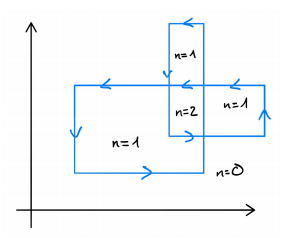
\includegraphics[width=0.3\textwidth]{img/windungszahl-1.png}
        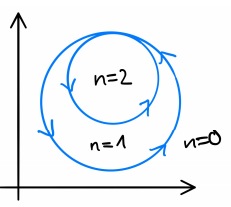
\includegraphics[width=0.3\textwidth]{img/windungszahl-2.png}
        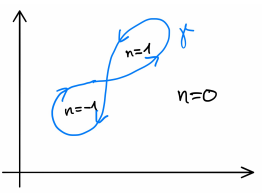
\includegraphics[width=0.3\textwidth]{img/windungszahl-3.png}
    \end{center}
    Ist \(\gamma\) die geschlossene Kurve \(\gamma(t) = z_0 + R \exp(2k \pi i t), k\in \Z\),
    so ist für jeden Punkt \(z\in C_R(z_0)\) 
    \[ n(\gamma, z) = k. \]
\end{karte}

\begin{karte}{Allgemeiner Satz von Cauchy}
    Ist \(U\subset \C\) einfach zusammenhängend und 
    \(\abb{f}{U}{\C}\) analytisch und \(\gamma\) eine 
    geschlossene Kurve in \(U\), so ist 
    \[ 2\pi i \; n(\gamma, z) f(z) = \int_\gamma \frac{f(\zeta)}{\zeta - z} d\zeta \]
    für jedes \(z\in U \setminus \Bild(\gamma)\).
\end{karte}

\begin{karte}{Regulär, Inneres, Äußeres}
    Eine geschlossene Kurve \(\gamma\) heißt regulär, falls 
    \[ n(\gamma, z) \in \set{0,1} \text{ für alle } z\in \C\setminus \Bild(\gamma). \]
    Wir nennen \(\set{ z\in \C: n(\gamma, z) = 1 }\) das Innere von \(\gamma\) 
    und \( z\in \C : n(\gamma, z) = 0 \) das Äußere von \(\gamma\).\\
    Das heißt für jede regulär geschlossene Kurve \(\gamma\) in einem einfach 
    zusammenhängenden Gebiet \(U\) und jede analytische Funktion 
    \(\abb{f}{U}{\C}\) gilt 
    \[ f(z) = \frac{1}{2\pi i} \int_\gamma \frac{f(\zeta)}{\zeta - z} \dx{\zeta} \]
    für alle \(z\) im Inneren von \(\gamma\).
\end{karte}